% ============================================================
%  example.tex
%  The following section contains minimal examples for common
%  IEEE TVCG elements such as figures, tables, equations and
%  references. These examples are for template purposes only
%  and should be removed before final submission.
% ============================================================



% ── Figure ──────────────────────────────────────────────────
\blindtext
\begin{figure}[!t]
    \centering
    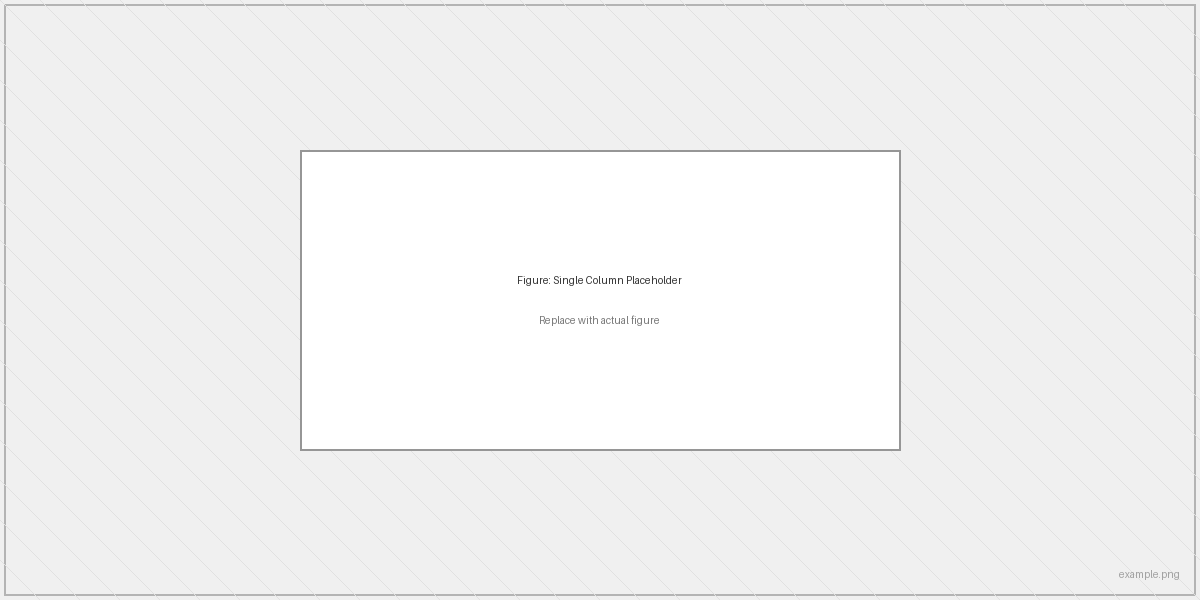
\includegraphics[width=\columnwidth]{figures/example.png}
    \caption{A single column figure example.}
    \label{fig:example}
\end{figure}

% ── Figure spanning both columns ────────────────────────────
\blindtext
\begin{figure*}[!t]
    \centering
    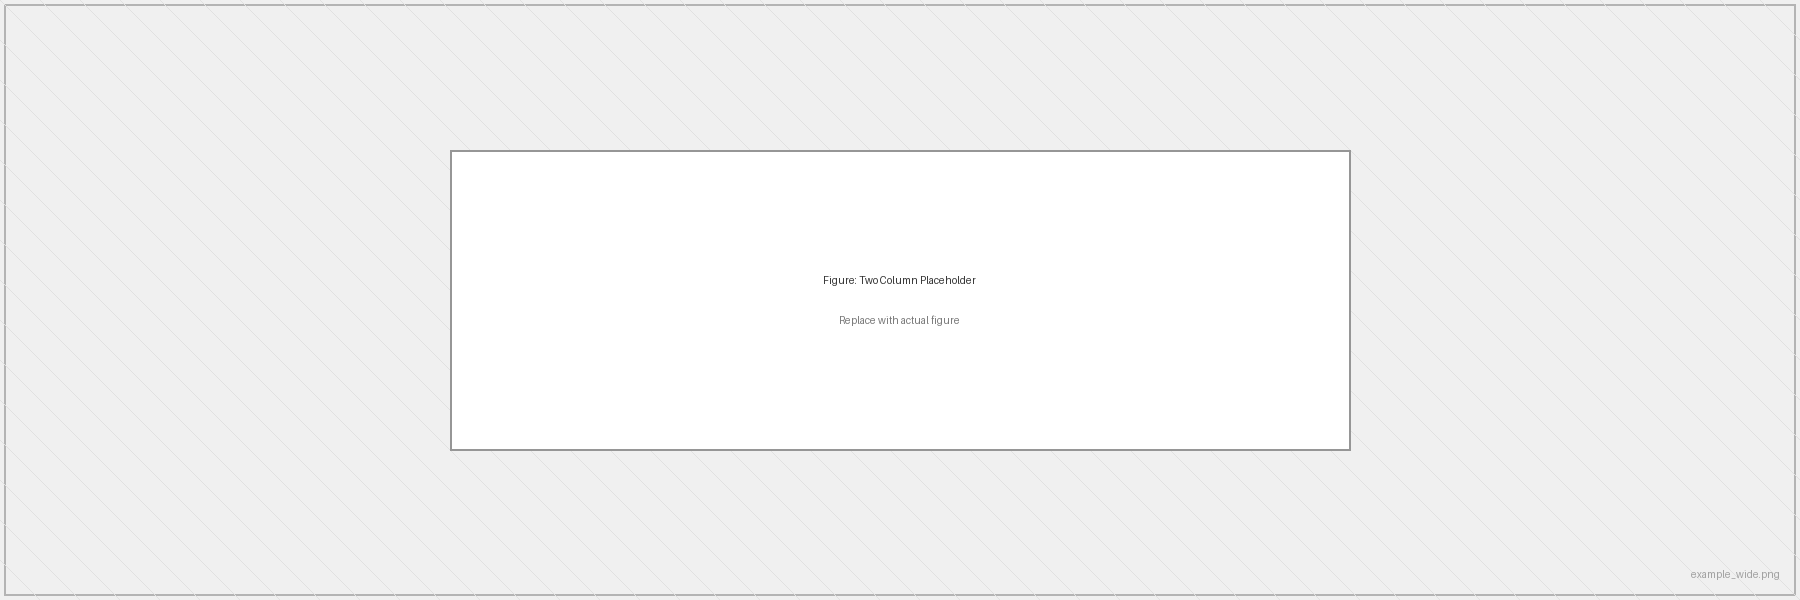
\includegraphics[width=\textwidth]{figures/example_wide.png}
    \caption{A two column figure example.}
    \label{fig:example_wide}
\end{figure*}

% ── Table ───────────────────────────────────────────────────
\blindtext
\begin{table}
    \caption{An Example Table}
    \label{tab:example}
    \centering
    \begin{tabular}{|c|c|c|}
        \hline
        Column A & Column B & Column C \\
        \hline
        Value 1  & Value 2  & Value 3  \\
        \hline
        Value 4  & Value 5  & Value 6  \\
        \hline
    \end{tabular}
\end{table}

% ── Equation ────────────────────────────────────────────────
\blindtext
\begin{equation}
    y = mx + b
    \label{eq:example}
\end{equation}

% ── References ──────────────────────────────────────────────
\blindtext
As shown in \cref{fig:example}, the results indicate...
\blindtext
As defined in \cref{eq:example}, the formula shows...
\blindtext
See \cref{tab:example} for an overview.
\blindtext
This has been demonstrated in prior work \cite{test}.
\blindtext
If you need multiple citations, you can use \cite{test, test, test}.